% !TEX TS-program = xelatex
% !TEX encoding = UTF-8 Unicode

% Tennessee Technological University
% ME4140 - Fall 2016 - Fall 2017 - ? - Fall 2019 - Fall 2020 
% Tristan Hill - August 08, 2020 - August 31, 2023
% Module 2 - Linux Basics
% Lecture 2 

\documentclass[fleqn]{beamer} % for presentation (has nav buttons at bottom)
\usepackage{../../ros_lecture}

\newcommand{\MNUM}{2\hspace{2mm}} % Module number
%\newcommand{\TNUM}{2\hspace{2mm}} % Topic number 
\newcommand{\moduletitle}{Linux Basics} % Titles and Stuff
\newcommand{\lecturetitle}{Lecture \MNUM - \moduletitle}  

\newcommand{\sectiontitleI}{What is Linux?} % More Titles and Stuff
\newcommand{\sectiontitleII}{A Brief History, Examples}
\newcommand{\sectiontitleIII}{Keyboard Shortcuts}
\newcommand{\sectiontitleIV}{The Terminal}
\newcommand{\sectiontitleV}{Tutorial 2 - Install ROS Noetic}

\author{ME4140 - ROS Workshop}
\title{\GD Module \MNUM - \moduletitle}
\date{Mechanical Engineering\vspc Tennessee Technological University}

\begin{document}
	
	\lstset{language=MATLAB,basicstyle=\ttfamily\small,showstringspaces=false}
	
	\frame{\titlepage \center\begin{framed}\Large \textbf{\lecturetitle}\end{framed} \vspace{5mm}}
	
	% Section 0 - Outline
	\frame{
		
		\large \textbf{\lecturetitle} \vspace{3mm}\\
	\begin{multicols}{2}
		\begin{itemize}
		
			\item \hyperlink{sectionI}{\color{black}\sectiontitleI}	\vspace{3mm} % Section I
			\item \hyperlink{sectionII}{\color{black}\sectiontitleII}	\vspace{3mm} % Section II
			\item \hyperlink{sectionIII}{\color{black}\sectiontitleIII}	\vspace{3mm} %Section III
			\item \hyperlink{sectionIV}{\color{black}\sectiontitleIV}	\vspace{3mm} %Section IV
			\item \hyperlink{sectionV}{\color{black}\sectiontitleV} %Section IV	
		
		\end{itemize}

		\hspace*{2mm}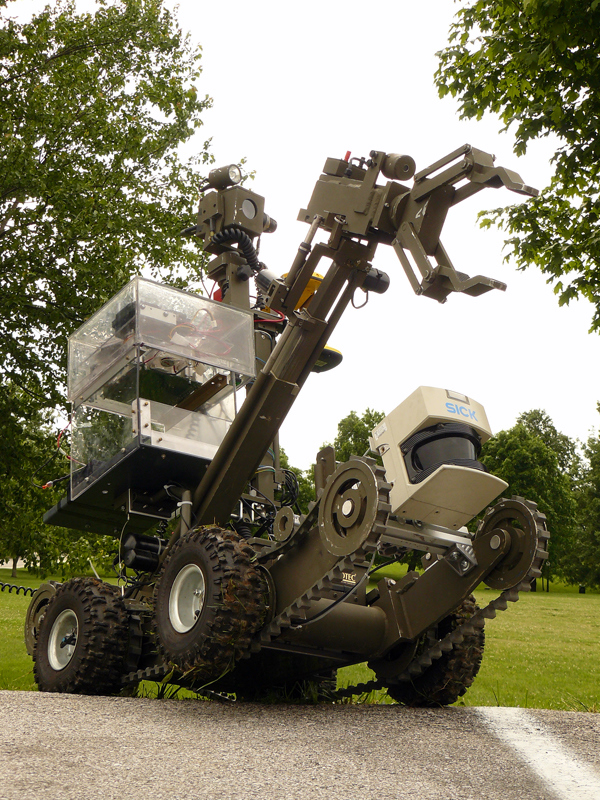
\includegraphics[scale=0.25]{AndrosII.jpg}
		
	\end{multicols}

}

\section{\sectiontitleI}

	% Section I - Frame I
	\begin{frame}[label=sectionI] \small
		\frametitle{\sectiontitleI}
		
\begin{itemize}
		\item {\it Just like Windows, iOS, and Mac OS, Linux is an operating system. In fact, one of the most popular platforms on the planet, Android, is powered by the Linux operating system. An operating system is software that manages all of the hardware resources associated with your desktop or laptop. To put it simply, the operating system manages the communication between your software and your hardware. Without the operating system (OS), the software wouldn't function.} - \href{https://www.linux.com/what-is-linux/}{LINUX.COM}  \vspc
        
            \end{itemize}
	\end{frame}

	% Section I - Frame II
	\begin{frame} \small
		\frametitle{\sectiontitleI}
			
			\hspace*{1cm}
\includegraphics[scale=.2]{Tux.png}\hspace{10mm}
\includegraphics[scale=.2]{UbuntuCoF.png}\hspace{10mm}
\includegraphics[scale=.15]{Debian_logo.png}

			Ubuntu is a \href{https://en.wikipedia.org/wiki/Linux_distribution}{distribution} of Linux. But there are many others. 
            \begin{itemize}
                \item 
                \item 
                \item 
            \end{itemize} 

            \btVFill
            {\tiny images: Wikimedia -\href{https://commons.wikimedia.org/w/index.php?curid=753970}{Tux}, \href{https://commons.wikimedia.org/wiki/File:UbuntuCoF.svg}{Ubuntu}, \href{https://commons.wikimedia.org/wiki/File:Debian_logo.png}{Debian}} 
	\end{frame}
		
\section{\sectiontitleII}	

	\begin{frame}[label=sectionII] \footnotesize
		\frametitle{\sectiontitleII}
			Once upon a time in California ...\vspc
            \begin{itemize}
                \item Unix was developed at Bell Labs (AT\&T) - Ken Thompson,  Dennis Richie - 1970 
                \item Berkely Software Distribution (BSD) - based on 6th edition Unix - \href{https://en.wikipedia.org/wiki/UNIX_System_Laboratories,_Inc._v._Berkeley_Software_Design,_Inc.}{lawsuit} - 1977
                \item Onyx Systems, \href{https://en.wikipedia.org/wiki/Sun_Microsystems}{Sun Microsystems} - single use UNIX microcomputer - 1980
                \item Richard Stallman started \href{https://en.wikipedia.org/wiki/GNU_Project}{GNU project} - \href{https://en.wikipedia.org/wiki/GNU_General_Public_License}{General Public License (GPL)} - 1983
                \item Intel Released \href{https://en.wikipedia.org/wiki/X86}{x86 microprocessor} - 1985
                \item Andrew Tanenbaum created MINIX for academic use - 1987
                \item Linus Torvalds began the \href{https://en.wikipedia.org/wiki/Linux_kernel}{Linux kernal} - 1991 

            \end{itemize} 
		
		\btVFill
    	\tiny{reference: \href{https://en.wikipedia.org/wiki/History_of_Linux}{Wikipedia}, \href{https://www.bell-labs.com/var/articles/invention-unix/}{Bell Labs}}	
            
	\end{frame}

	\begin{frame}[label=sectionII] \footnotesize
		\frametitle{\sectiontitleII}
		
		What is Linux used for? \vspcc

		\begin{itemize}

			\item The Internet - in 2015 96\% worlds webservers \href{https://www.zdnet.com/home-and-office/networking/can-the-internet-exist-without-linux/}{ran on Linux} - \href{https://www.nginx.com/}{NGINX}, \href{https://www.apache.org/}{Apache}

			\item \href{https://en.wikipedia.org/wiki/Smart_device}{Smart Devices} - Web Enabled Technology

			\item NASA \href{https://www.nas.nasa.gov/hecc/resources/pleiades.html}{Pleiades Supercomputer} - \href{https://www.nas.nasa.gov/hecc/support/kb/vnc-a-faster-alternative-to-x11_257.html}{runs on Linux}

			\item Automobiles - Toyota, Mazda, Mercedez-Benv, Volkswagen - \href{https://www.automotivelinux.org/}{Automotive Grade Linux}

			\item Robotics - \href{https://bostondynamics.com/}{Boston Dynamics} - \href{https://www.universal-robots.com/}{Universal Robotics}


		\end{itemize}

	\end{frame}
	
		


\section{\sectiontitleIII}	
	% Section III - Frame I
	\begin{frame}[label=sectionIII] \small
		\frametitle{\sectiontitleIII}
		Press \WinKey and type {\it Keyboard Shortcuts} to list shortcuts in Ubuntu.
		
		\begin{multicols}{2}
		
		\renewcommand{\arraystretch}{1.4}
		\begin{tabular}{|c|c|}\hline
			Function & Shortcut \\ \hline
			Launcher &\WinKey  \\
			New Terminal &\CTRLKey+\ALTKey+T \\
			Abort Process &\\
		    Switch Windows &\\
			Close Window & \\
			Rename &\\
			New Folder & \\ \hline						
		\end{tabular}
			
		\hspace{10mm}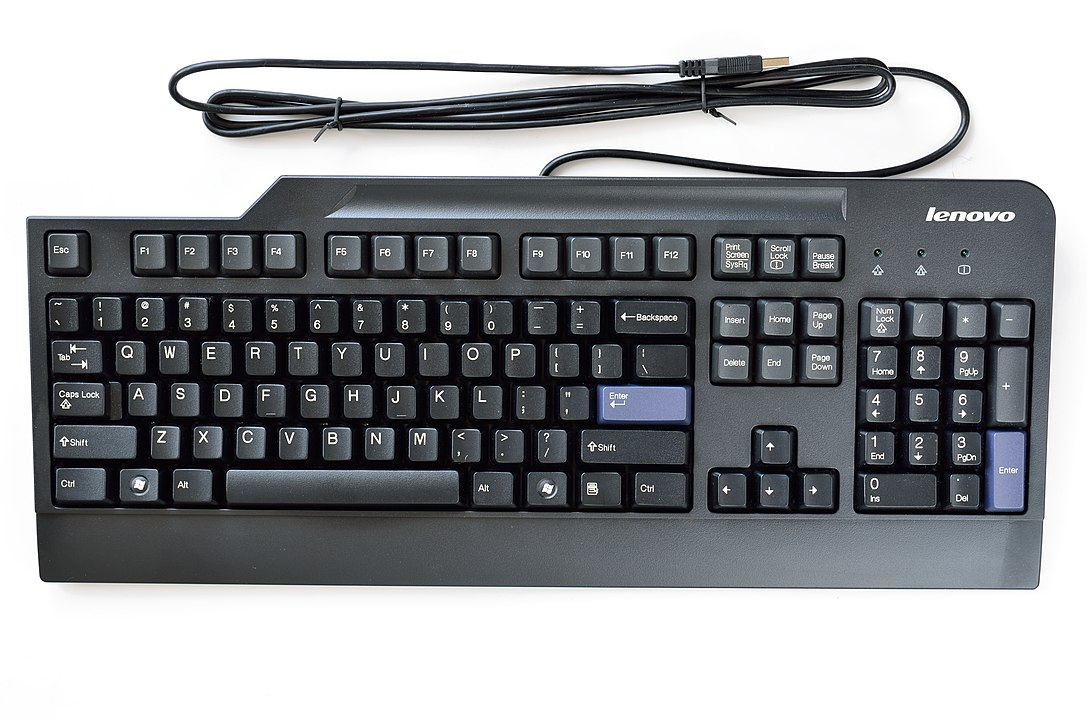
\includegraphics[scale=.10]{lenovo_keyboard.jpg} 
       	       
        \end{multicols}

	\end{frame}      
	
\section{\sectiontitleIV}	
	% Section IV - Frame I
	\begin{frame}[label=sectionIV] \small
		\frametitle{\sectiontitleIV}    
          The {\it Terminal} is a text based interface to the computer.\vspace{2mm}\\ Press \CTRLKey+\ALTKey+T to open a new terminal. \vspace{3mm}\\      
                \begin{multicols}{2}
		
		\renewcommand{\arraystretch}{1.4}
		\begin{tabular}{|c|c|}\hline
				Function & Command \\ \hline
			 Change Directory & cd  \\ 
			List Directory & ls \\  
			Copy File& cp \\ 
			Remove File& rm  \\ 
			Abort Process& \CTRLKey + C  \\ 
			Clear Terminal& \CTRLKey + L  \\ \hline
				
		\end{tabular}
			
		\hspace{10mm}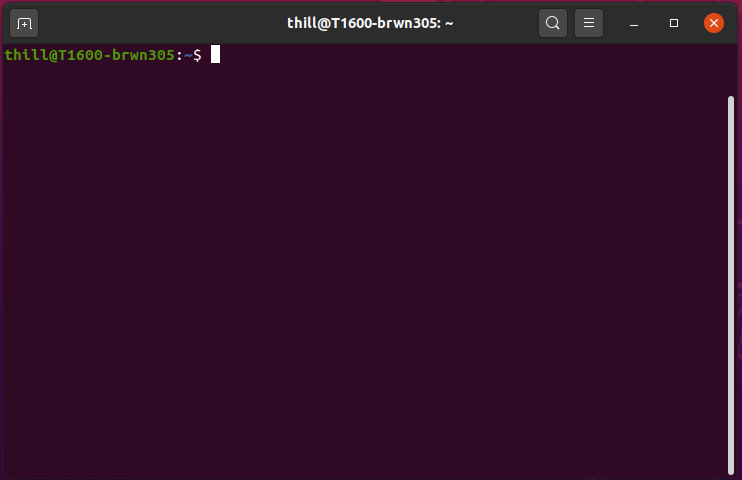
\includegraphics[scale=.20]{ubuntu_terminal.png}  
       	       
        \end{multicols}

       	                       
                
		\end{frame}
		


\section{\sectiontitleV}	
	% Section V - Frame I
	            \begin{frame}[label=sectionV] \small
		\frametitle{\sectiontitleV}    
	
 \setbeamertemplate{itemize items}[triangle]
                \begin{itemize}

					\item {\bf Overview:} ROS runs on Linux! Now that Ubuntu is setup you need to install ROS. 		

					\item {\bf Assignment:} Complete the tutorial \href{https://github.com/thillRobot/ros_workshop/blob/main/module2/tutorial2_install_ros/tutorial2_install_ros.md}{\it Tutorial2 Install ROS} on ilearn. Your new system must have ROS \rosdistro \hspace{1mm} installed.
                    
                    \item {\bf Deliverable:} Write a one to two paragraph summary of what you accomplished and what you struggled with the most. Include an image of a terminal after the {\it roscore} command. 
    
                    \item {\bf Next Week:} After completion of Module 2, you will be ready to start using ROS. You will begin with a simple turtle robot simulator. \vspc
                               
                \end{itemize}
		\end{frame}

\end{document}


